\documentclass[12pt,a4paper]{article}

\usepackage[T1,T2A]{fontenc}
\usepackage[utf8]{inputenc}
\usepackage[english, russian]{babel}
\usepackage{indentfirst}
\usepackage{misccorr}
\usepackage{graphicx}
\usepackage{amsmath}
\usepackage{graphicx}
\usepackage{float}
\usepackage[left=20mm,right=10mm, top=20mm,bottom=20mm,bindingoffset=0mm]{geometry}

\setlength{\parskip}{6pt}
\DeclareGraphicsExtensions{.png}

\begin{document}

    \begin{titlepage}
        \begin{center}
            \large
            Санкт-Петербургский политехнический университет\\Петра Великого\\
            \vspace{0.5cm}
            Институт прикладной математики и механики\\
            \vspace{0.25cm}
            Кафедра «Прикладная математика»
            \vfill
            \textsc{\LARGE\textbf{Отчет по лабораторной работе №5}}\\[5mm]
            \Large
            по дисциплине\\"Математическая статистика"
        \end{center}
        \vfill
        \begin{tabular}{l p{175} l}
            Выполнила студентка\\группы 3630102/80201 && Деркаченко Анна Олеговна
            \vspace{0.25cm}
            \\Проверил\\доцент, к.ф.-м.н. && Баженов Александр Николаевич
        \end{tabular}
        \vfill
        \begin{center}
            Санкт-Петербург\\2021 г.
        \end{center}
    \end{titlepage}

\newpage
\begin{center}
    \tableofcontents
    \setcounter{page}{2}
\end{center}
\newpage
\begin{center}
    \listoffigures
\end{center}

\newpage
\section{Постановка задачи}
Дано нормальное двумерное распределение $N(x,y,0,0,1,1,\rho)$.

Необходимо:
\begin{enumerate}
    \item Сгенерировать выборки размером 20, 60 и 100 элементов с коэффициентом корреляции $\rho$, равным 0, 0.5, 0.9
    \item Сгенерировать выборки 1000 раз и вычислить среднее значение, среднее значение квадрата и дисперсию коэффициентов корреляции Пирсона, Спирмена и квадрантного коэффициента корреляции
    \item Повторить все вычисления для смеси нормальных распределений:
        \begin{equation}
	        f(x,y)=0.9N(x,y,0,0,1,1,0.9)+0.1N(x,y,0,0,10,10,-0.9)
        \end{equation}
    \item Изобразить сгенерированные точки на плоскости и нарисовать эллипс равновероятности
\end{enumerate}

\section{Теория}
\subsection{Двумерное нормальное распределение}
Двумерная случайная величина $(X,Y)$ называется \textit{распределённой нормально} (или просто нормальной), если её плотность вероятности определена формулой
\begin{equation}
    N(x,y,\bar{x},\bar{y},\sigma_x,\sigma_y,\rho)=\frac{1}{2\pi\sigma_x\sigma_y\sqrt{1-\rho^2}}\times\exp{
    \begin{Bmatrix}
        -\frac{1}{2(1-\rho^2)}
        \begin{bmatrix}
            \frac{(x-\bar{x})^2}{\sigma_x^2}-2\rho\frac{(x-\bar{x})(y-\bar{y})}{\sigma_x\sigma_y}+\frac{(y-\bar{y})^2}{\sigma_y^2}
        \end{bmatrix}
    \end{Bmatrix}
    }
\end{equation}

Компоненты $X,Y$ двумерной нормальной случайной величины также распределены нормально с математическими ожиданиями $\bar{x}$,$\bar{y}$ и средними квадратическими отклонениями $\sigma_{x},\sigma_{y}$ соответственно. Параметр $\rho$ называется коэффициентом корреляции.

\subsection{Корреляционный момент (ковариация) и коэффициент корреляции}
\textit{Корреляционный момент (ковариация)} двух случайных величин $X$ и $Y$ - математическое ожидание произведения отклонений этих случайных величин от их математических ожиданий:
\begin{equation}
    K=cov(X,Y)=M[(X-\bar{x})(Y-\bar{y})]
\end{equation}

\textit{Коэффициент корреляции $\rho$} двух случайных величин $X$ и $Y$ - отношение их корреляционного момента к произведению их средних квадратических отклонений:
\begin{equation}
    \rho=\frac{K}{\sigma_x\sigma_y}
\end{equation}

\textit{Коэффициент корреляции} — нормированная числовая характеристика, являющаяся мерой близости зависимости между случайными величинами к линейной.

\subsection{Выборочные коэффициенты корреляции}
\subsubsection{Выборочный коэффициент корреляции Пирсона}
Пусть по выборке значений $\{x_i,y_i\}^n_1$ двумерной с.в. $(X,Y)$ требуется оценить коэффициент корреляции $\rho=\frac{cov(X,Y)}{\sqrt{DXDY}}$. Естественной оценкой для $\rho$ служит его статистический аналог в виде выборочного коэффициента корреляции, предложенного К.Пирсоном:
\begin{equation}
    r=\frac{\frac{1}{n}\sum{(x_i-\bar{x})(y_i-\bar{y})}}{\sqrt{\frac{1}{n}\sum{(x_i-\bar{x})^2}\frac{1}{n}\sum{(y_i-\bar{y})^2}}}=\frac{K}{s_Xs_Y},
\end{equation}
где $K,s^2_X,s^2_Y$ — выборочные ковариация и дисперсии с.в. $X$ и $Y$

\subsubsection{Выборочный квадрантный коэффициент корреляции}
Кроме выборочного коэффициента корреляции Пирсона, существуют и другие оценки степени взаимосвязи между случайными величинами. К ним относится выборочный квадрантный коэффициент корреляции:
\begin{equation}
    r_Q=\frac{(n_1+n_3)-(n_2+n_4)}{n},
\end{equation}
где $n_1,n_2,n_3,n_4$ - количества точек с координатами $x_i,y_i$, попавшими соответственно в I, II, III, IV квадранты декартовой системы с осями $x'=x-medx,y'=y-medy$ и с центром в точке с координатами $(medx,medy)$

\subsubsection{Выборочный коэффициент ранговой корреляции Спирмена}
Если объект обладает не одним, а двумя качественными признаками — переменными $X$ и $Y$ , то для исследования их взаимосвязи используют выборочный коэффициент корреляции между двумя последовательностями рангов этих признаков.

Обозначим ранги, соотвествующие значениям переменной $X$, через $u$, а ранги, соотвествующие значениям переменной $Y$, — через $v$.

Выборочный коэффициент ранговой корреляции Спирмена определяется как выборочный коэффициент корреляции Пирсона между рангами $u,v$ переменных $X,Y:$
\begin{equation}
    r_S=\frac{\frac{1}{n}\sum{(u_i-\bar{u})(v_i-\bar{v})}}{\sqrt{\frac{1}{n}\sum{(u_i-\bar{u})^2}\frac{1}{n}\sum{(v_i-\bar{v})^2}}},
\end{equation}
где $\bar{u}=\bar{v}=\frac{1+2+...+n}{n}=\frac{n+1}{2}$ — среднее значение рангов

\subsection{Эллипсы рассеивания}
При сечении поверхности функции нормального двумерного распределения плоскостями, паралелльными плоскости $xOy$, получаются эллипсы:
\begin{equation}
    \frac{(x-\bar{x})^2}{\sigma_x^2}-2\rho\frac{(x-\bar{x})(y-\bar{y})}{\sigma_x\sigma_y}+\frac{(y-\bar{y})^2}{\sigma_y^2}=const
\end{equation}

Центр эллипса находится в точке с координатами $(\bar{x},\bar{y})$, а направления осей симметрии эллипса составляют с осью $Ox$ углы, определяемые уравнением:
\begin{equation}
    \tg(2\alpha)=\frac{2\rho\sigma_x\sigma_y}{\sigma_x^2-\sigma_y^2}
\end{equation}

Это уравнение дает два значения углов: $\alpha$ и $\alpha_1$, различающиеся на $\frac{\pi}{2}$.

Таким образом, ориентация эллипса относительно координатных осей находится в прямой зависимости от коэффициента корреляции $\rho$ системы $(X,Y)$. Если величины не коррелированны (т.е. в данном случае и независимы), то оси симметрии эллипса параллельны координатным осям, в противном случае они составляют с координатными осями некоторый угол.

Пересекая поверхность распределения плоскостями, параллельными плоскости $xOy$, и проектируя сечения на плоскость $xOy$ мы получим целое семейство подобных и одинаково расположенных эллипсов с общим центром $(\bar{x},\bar{y})$. Во всех точках каждого из таких эллипсов плотность данного распределения постоянна. Поэтому такие эллипсы называются эллипсами равной плотности или, короче эллипсами рассеивания. Общие оси всех эллипсов рассеивания называются главными осями рассеивания.

\section{Реализация}
Реализация лабораторной работы проводилась на языке Python в среде разработки PyCharm c использованием дополнительных библиотек:
\begin{itemize}
    \item scipy
    \item numpy
    \item matplotlib
    \item statistics
    \item statsmodels
\end{itemize}

Исходный код лабораторной работы размещен в GitHub-репозитории.

URL: https://github.com/derkanw/Mathstat/tree/main/lab5

\section {Результаты}
\subsection{Вычислительные характеристики распределения}
\begin{table}[H]
    \centering
    \begin{tabular}{|c|c|c|c|}
        \hline
        & $r$ & $r_S$ & $r_Q$\\\hline
        $\rho=0$ & & &\\\hline
        $E(z)$ & -0.0166 & -0.0188 & 0.0\\\hline
        $E(z^2)$ & 0.0232 & 0.0245 & 0.04\\\hline
        $D(z)$ & 0.0514 & 0.053 & 0.0515\\\hline
        \hline
        $\rho=0.5$ & & &\\\hline
        $E(z)$ & 0.5061 & 0.4677 & 0.4\\\hline
        $E(z^2)$ & 0.2562 & 0.2187 & 0.16\\\hline
        $D(z)$ & 0.0334 & 0.0373 & 0.0501\\\hline
        \hline
        $\rho=0.9$ & & &\\\hline
        $E(z)$ & 0.9037 & 0.8797 & 0.8\\\hline
        $E(z^2)$ & 0.8167 & 0.7739 & 0.64\\\hline
        $D(z)$ & 0.0027 & 0.005 & 0.0289\\\hline
    \end{tabular}
    \caption{Характеристики распределения размерностью n = 20}
\end{table}

\begin{table}[H]
    \centering
    \begin{tabular}{|c|c|c|c|}
        \hline
        & $r$ & $r_S$ & $r_Q$\\\hline
        $\rho=0$ & & &\\\hline
        $E(z)$ & 0.7933 & 0.7579 & 0.6\\\hline
        $E(z^2)$ & 0.6294 & 0.5744 & 0.36\\\hline
        $D(z)$ & 0.0091 & 0.0136 & 0.0386\\\hline
        \hline
        $\rho=0.5$ & & &\\\hline
        $E(z)$ & 0.0016 & 0.0014 & 0.0\\\hline
        $E(z^2)$ & 0.0085 & 0.0082 & 0.0044\\\hline
        $D(z)$ & 0.0183 & 0.0181 & 0.0167\\\hline
        \hline
        $\rho=0.9$ & & &\\\hline
        $E(z)$ & 0.5091 & 0.4894 & 0.3333\\\hline
        $E(z^2)$ & 0.2592 & 0.2395 & 0.1111\\\hline
        $D(z)$ & 0.0101 & 0.0113 & 0.015\\\hline
    \end{tabular}
    \caption{Характеристики распределения размерностью n = 60}
\end{table}

\begin{table}[H]
    \centering
    \begin{tabular}{|c|c|c|c|}
        \hline
        & $r$ & $r_S$ & $r_Q$\\\hline
        $\rho=0$ & & &\\\hline
        $E(z)$ & 0.9029 & 0.8886 & 0.7333\\\hline
        $E(z^2)$ & 0.8153 & 0.7897 & 0.5378\\\hline
        $D(z)$ & 0.0006 & 0.001 & 0.0087\\\hline
        \hline
        $\rho=0.5$ & & &\\\hline
        $E(z)$ & 0.7953 & 0.7736 & 0.6\\\hline
        $E(z^2)$ & 0.6324 & 0.5985 & 0.36\\\hline
        $D(z)$ & 0.0026 & 0.0037 & 0.0119\\\hline
        \hline
        $\rho=0.9$ & & &\\\hline
        $E(z)$ & -0.0089 & -0.0078 & 0.0\\\hline
        $E(z^2)$ & 0.005 & 0.005 & 0.0064\\\hline
        $D(z)$ & 0.0107 & 0.0105 & 0.0096\\\hline
    \end{tabular}
    \caption{Характеристики распределения размерностью n = 100}
\end{table}

\begin{table}[H]
    \centering
    \begin{tabular}{|c|c|c|c|}
        \hline
        & $r$ & $r_S$ & $r_Q$\\\hline
        $n=20$ & & &\\\hline
        $E(z)$ & 0.4987 & 0.479 & 0.32\\\hline
        $E(z^2)$ & 0.2487 & 0.2294 & 0.1024\\\hline
        $D(z)$ & 0.0061 & 0.0069 & 0.0088\\\hline
        \hline
        $n=60$ & & &\\\hline
        $E(z)$ & 0.9006 & 0.889 & 0.72\\\hline
        $E(z^2)$ & 0.811 & 0.7904 & 0.5184\\\hline
        $D(z)$ & 0.0004 & 0.0006 & 0.0054\\\hline
        \hline
        $n=100$ & & &\\\hline
        $E(z)$ & 0.7917 & 0.7734 & 0.56\\\hline
        $E(z^2)$ & 0.6268 & 0.5981 & 0.3136\\\hline
        $D(z)$ & 0.0015 & 0.0021 & 0.0071\\\hline
    \end{tabular}
    \caption{Смесь нормальных распределений}
\end{table}

\subsection{Эллипсы рассеивания}
\begin{figure}[H]
    \centering
    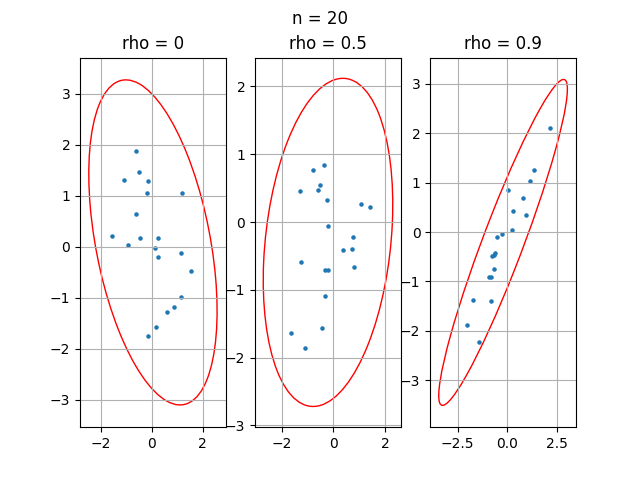
\includegraphics[scale=0.85]{images/ellipses20.png}
    \caption{Эллипс рассеивания для 20 элементов}
\end{figure}

\begin{figure}[H]
    \centering
    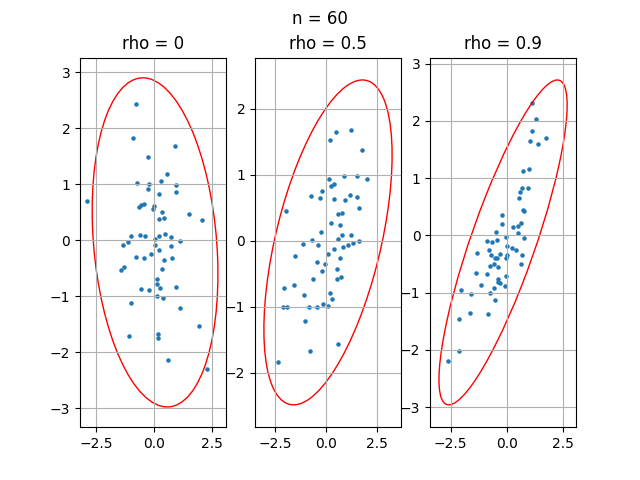
\includegraphics[scale=0.85]{images/ellipses60.png}
    \caption{Эллипс рассеивания для 60 элементов}
\end{figure}

\begin{figure}[H]
    \centering
    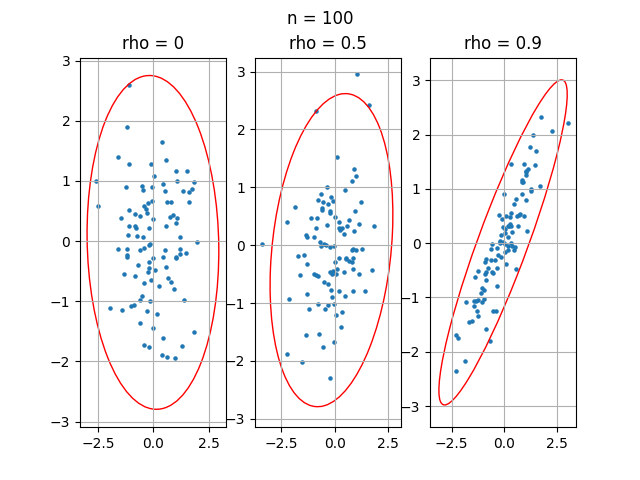
\includegraphics[scale=0.85]{images/ellipses100.png}
    \caption{Эллипс рассеивания для 100 элементов}
\end{figure}

\section{Обсуждение}
Исходя из таблиц характеристик распределений разных размерностей и смеси распределений, можно можно сделать вывод, что значения $E(z),E(z^2)$ для величин $r,r_S,r_Q$ в большинстве случаев подчиняются соотношению $r>r_S>r_Q$. А для дисперсии наблюдается обратное: $r<r_S<r_Q$. При этом с ростом размерности выборки дисперсия уменьшается для более приближающегося к нулю коэффициента корреляции Стоит также сказать, что дисперсии для смеси распределений имеют меньшие значения по сравнению с соответствующими показателями для обычного распределения.

На графиках эллипсов рассеивания можно наблюдать, что почти все элементы выборки попадают в границы данных эллипсов, исходя из чего можно сделать вывод, что полученный результат можно назвать соответствующим его теоретической оценке. При этом достаточно большая часть значений концентрируется в центре эллипсов, что подтверждает вывод о теоретическом значении центра эллипса, координаты которого представляются в виде среднего для исследуемых величин $X,Y$.
\end{document}
